% Enable warnings about problematic code
\RequirePackage[l2tabu, orthodox]{nag}

\PassOptionsToPackage{utf8}{inputenc}
\PassOptionsToPackage{T1}{fontenc}
\PassOptionsToPackage{ngerman, american}{babel}

\documentclass{presentation}

\title[Fast Word Prediction using Top-K Joins]{\mbox{Fast and Non-Approximative} \mbox{Language Model Prefixqueries} \mbox{for Word Prediction using} \mbox{Top-k Joining Techniques}}
\subtitle{Bachelor Thesis}
\author[Lukas Schmelzeisen]{\texorpdfstring{Lukas Schmelzeisen\\\textcolor{Maroon}{\scriptsize{\texttt{\href{mailto:lukas@uni-koblenz.de}{\nolinkurl{lukas@uni-koblenz.de}}}}}}{Lukas Schmelzeisen}}
\date{August 6, 2015}
\institute[Institute for Web Science and Technologies]{Institute for Web Science and Technologies,\\University of Koblenz-Landau}

% For resizing
\usepackage{graphicx}

% For figures, equation explanation
\usepackage{standalone}
\usepackage{tikz}
\usepackage{pgfplots}
\pgfplotsset{compat = 1.12}
\usetikzlibrary{tikzmark, positioning}

\usepackage{appendixnumberbeamer}

\addbibresource{bibliography.bib}

\begin{document}

\begin{frame}[plain]
  \maketitle
\end{frame}

\begin{frame}[plain]
  \frametitle{Outline}

  \tableofcontents
\end{frame}

% ==============================================================================
\section{Next Word Prediction}
\subsection{}

\begin{frame}
  \frametitle{What is Next Word Prediction?}

  \onslide<2->{
    \begin{center}
      \LARGE Demo
    \end{center}}
\end{frame}


\begin{frame}
  \frametitle{Benefits of good Word Prediction}

  \large
  \begin{itemize}
    \item Faster typing
    \item Spelling
    \item \ldots
  \end{itemize}
\end{frame}

\begin{frame}
  \frametitle{Next Word Prediction}

  \LARGE
  \begin{equation*}
    \only<1-3>{\phantom{_{p}}\NWP{\tikzmark{hist1_fst}h} = \Argmax{\mathclap{\substack{w \in \Vocab\\\phantom{p \: \text{prefix of} \: w}}}}\tikzmark{vocab_fst} \Prob{\tikzmark{w_fst}w}{\tikzmark{hist2_fst}h}}
    \only<4- >{\NWP[\tikzmark{prefix}p]{\tikzmark{hist1_snd}h} = \Argmax{\mathclap{\substack{w \in \Vocab,\\p \: \text{prefix of} \: w}}}\tikzmark{vocab_snd} \Prob{\tikzmark{w_snd}w}{\tikzmark{hist2_snd}h}}
  \end{equation*}

  \large
  \begin{tikzpicture}[
    remember picture,
    overlay,
    expl/.style = {draw = Maroon, rounded corners, thick},
    arrow/.style = {Maroon, thick, ->, >=latex}
  ]
    \node<2->[expl]
      (hist_expl) at (2,3.5cm) {history of entered words};
    \node<3->[expl]
      (vocab_expl) at (8.5,-1.5cm) {for each word in vocabulary};
    \node<4->[expl, align=center]
      (prefix_expl) at (2.5,-1cm) {entered prefix of\\intended word};
    \LARGE % restore equation size so font relative units are correct
    \draw<2-3>[arrow] (hist_expl.south)   to [out=270, in=100] ([xshift= 0.2em, yshift= 2.0ex]{pic cs:hist1_fst});
    \draw<2-3>[arrow] (hist_expl.east)    to [out=  0, in=100] ([xshift= 0.2em, yshift= 2.0ex]{pic cs:hist2_fst});
    \draw<4- >[arrow] (hist_expl.south)   to [out=270, in=100] ([xshift= 0.2em, yshift= 2.0ex]{pic cs:hist1_snd});
    \draw<4- >[arrow] (hist_expl.east)    to [out=  0, in=100] ([xshift= 0.2em, yshift= 2.0ex]{pic cs:hist2_snd});
    \draw<3  >[arrow] (vocab_expl.north)  to [out= 90, in=  0] ([xshift=-0.7em, yshift=-1.3ex]{pic cs:vocab_fst});
    \draw<3  >[arrow] (vocab_expl.north)  to [out= 90, in=270] ([xshift= 0.4em, yshift=-0.6ex]{pic cs:w_fst});
    \draw<4- >[arrow] (vocab_expl.north)  to [out= 90, in=  0] ([xshift=-0.7em, yshift=-1.3ex]{pic cs:vocab_snd});
    \draw<4- >[arrow] (vocab_expl.north)  to [out= 90, in=270] ([xshift= 0.4em, yshift=-0.6ex]{pic cs:w_snd});
    \draw<4- >[arrow] (prefix_expl.north) to [out= 90, in=270] ([xshift= 0.2em, yshift=-0.9ex]{pic cs:prefix});
  \end{tikzpicture}
\end{frame}

\begin{frame}
  \frametitle{How to find probabilities?}

  \begin{center}
    \LARGE $\Prob{w}{h}$ ?
  \end{center}

  \vspace{1cm}

  \onslide<2->{
    \large
    Solution: use Language Models!
  }

  \vspace{1cm}

  \onslide<3->{
    \large
    We will use two state-of-the-art Language Models:
    \begin{itemize}
      \item Modified Kneser Ney Smoothing\\[-0.4ex]{\small\parencite{ChenGoodman1999}}
      \item Generalized Language Model\\[-0.4ex]{\small\parencite{Pickhardt2014}}
    \end{itemize}
  }
\end{frame}


% ==============================================================================
\section{Language Models}
\subsection{}

\begin{frame}
  \frametitle{Express as Weighted Sums}

  \LARGE
  \begin{equation*}
    \Prob{w}{h} = \sum_{i = 1}^{N} \SumWeight_i^h \; \SumArg_i^h(w)
  \end{equation*}
\end{frame}

% ==============================================================================
\section{Top-k Joining Techniques}
\subsection{}

% ==============================================================================
\appendix
\begin{frame}[plain]
  \frametitle{So long, and thanks for all the fish}
\end{frame}

\section{References}
\subsection{}
\begin{frame}[t, allowframebreaks]
  \frametitle{References}

  \printbibliography[heading = none]
\end{frame}

\end{document}
